%!TeX program = XeLaTeX
\documentclass[12pt, a4paper, twocolumn]{article} 
%\usepackage[no-math]{xeCJK} %For Traditional Chinese in XeLaTeX
%\setCJKmainfont{MingLiU} %For Traditional Chinese in XeLaTeX
%\setCJKsansfont{Microsoft JhengHei} %For Traditional Chinese in XeLaTeX

% *** MISC UTILITY PACKAGES ***
%
\usepackage[english]{babel}
\usepackage{placeins}
%\usepackage{ifpdf}
% Heiko Oberdiek's ifpdf.sty is very useful if you need conditional
% compilation based on whether the output is pdf or dvi.
% usage:
% \ifpdf
%   % pdf code
% \else
%   % dvi code
% \fi

% *** GRAPHICS RELATED PACKAGES ***
%
%\usepackage[pdftex]{graphicx}
\usepackage{graphicx}
% declare the path(s) where your graphic files are
\graphicspath{{./Figures/}{../Figures/}{../}{../../}} 
% and their extensions so you won't have to specify these with
% every instance of \includegraphics
\DeclareGraphicsExtensions{.pdf,.jpeg,.png}

% *** MATH PACKAGES ***
%
\usepackage[cmex10]{amsmath}

%\interdisplaylinepenalty=2500
% after loading amsmath to restore such page breaks as IEEEtran.cls normally
% does. amsmath.sty is already installed on most LaTeX systems. The latest
% version and documentation can be obtained at:
% http://www.ctan.org/tex-archive/macros/latex/required/amslatex/math/
\usepackage{amssymb,amsfonts} %Added to get math
\usepackage{amsthm} % Added to get theorems
\usepackage{mathtools} % Added to get \mathclap working
%\usepackage{bbold} % Defines \mathbb{} for numbers but also changes to a sans serif font for captial letters
%\usepackage{doublestroke} % Defines \mathds{} which I use to get symbol for vector with ones (Too complicated installation so skip)
\usepackage{bbm} % Defines \mathbbm{} which I use to get symbol for vector with ones


% *** FLOAT PACKAGES ***
%
\usepackage{paralist} % Inline list used in box
\usepackage{lipsum,framed} % Needed to create box and my comments
\usepackage{color} %Needed for color, the option usenames,dvipsnames will define a set of basic colors.
\usepackage[table]{xcolor} %Needed to color rows in table
%\usepackage[config, font={small}, labelfont={bf}, margin={3mm}]{caption, subfig} %Modifies the look of the captions of floats (may cause conflict with memoir class)
%\usepackage[config, margin={3mm}, font={small}, labelfont={bf}]{caption}%Modifies the look of the captions of floats (may cause conflict with memoir class)
\usepackage{subcaption}
%\usepackage{rotating} %Add to rotate figures and tables in PDF file
%\usepackage{filecontents} %Adds ability to compile separate files from within tex code, used for Practical_collinearity_for_column_uncertainty_proof_illustration_All.pdf generation

% Tabular packages
%\usepackage{longtable}
%\usepackage{multirow} % Add to get multirow working in tabular
%\usepackage{arydshln} %Add to get dashed lines working in tabular
%\usepackage{booktabs} %Commands for enhancing quality of tables
%\usepackage{adjustbox} %Handy for resizing tables
\usepackage{diagbox} % split cell daigonally
\usepackage[para,online,flushleft]{threeparttable}

\usepackage{ifdraft} %Enables \ifdraft{draft case}{final case} where things automatically are turned on and off depending on draft status.
\usepackage{comment} %Used to get comments turned on or off.
\usepackage{xspace} %Added to get automatic spacing after e.g., etc.
\usepackage{setspace} % Added to get todo boxes working (needed for \singlespacing) N
%\usepackage{makeidx} %Used to generate index
%\makeindex %Needed to tell Latex to make the index
%% Need to run command makeindex %.idx 
%\usepackage[intoc]{nomencl} %Can be used to generate abbreviations list but produces multiple entries if defined more than once, so glossaries is recomended.
%\renewcommand{\nomname}{Abbreviations}
%\makenomenclature %Needed to tell Latex to make the abbreviations list
%% Need to run command makeindex %.nlo -s nomencl.ist -o %.nls
%makeindex Nordling_PhD_thesis_main.nlo -s nomencl.ist -o Nordling_PhD_thesis_main.nls
\usepackage{etex} % Added to be able to use tikz
\usepackage{tikz} % Added to get todo boxes (must be after graphicx and color)
%\usepackage[final]{microtype} %Function unknown added by Per Sahlholm
%\usepackage{marvosym} %Function unknown added by Per Sahlholm
%\usepackage[table]{xcolor} %Function unknown added by Per Sahlholm causes option clash.
\usepackage[final]{pdfpages} %Package for inserting PDF documents in generated document.
\usepackage{enumitem} %Change numbering in lists

% *** PDF, URL AND HYPERLINK PACKAGES ***
%
\usepackage{url}
% url.sty was written by Donald Arseneau. It provides better support for
% handling and breaking URLs. url.sty is already installed on most LaTeX
% systems. The latest version and documentation can be obtained at:
% http://www.ctan.org/tex-archive/macros/latex/contrib/url/
% Basically, \url{my_url_here}.
% Special hack below to break the damn URL!
\def\UrlBreaks{\do\.\do\@\do\\\do\/\do\!\do\_\do\|\do\;\do\>\do\]%
	\do\)\do\,\do\?\do\'\do+\do\=\do\#\do\i\do\m\do\t\do\a\do\x}%
\urlstyle{rm} %
\usepackage[bookmarks=true,bookmarksnumbered=true,hypertexnames=true,breaklinks=true,colorlinks=true]{hyperref} %Needed for showing hyperlinks in PDF, \url tags and hyperrefs. Need to be loaded last of all packages. pagebackref adds page numbers in the bibliography and links to the positions in the document where you actually cite them (If I add pagebackref=true then I get many errors)
%\usepackage[bookmarks=true,bookmarksnumbered=true,hypertexnames=true,breaklinks=true,colorlinks=false,pdfborder={0 0 0}]{hyperref} % Removes colors from hyperrefs
\hypersetup{
	pdfauthor = {Torbj\"{o}rn E. M. Nordling},
	pdftitle = {Literature Review},
	pdfsubject = {Research Proposal},
	pdfkeywords = {Research Proposal}}

% *** User specific macros ***
%
\usepackage{../macros_tn} %Loads all my macros

%\usepackage{epigraph}
%\setlength{\epigraphwidth}{0.9\columnwidth}
%\newcommand{\epi}[2]{
%	\begin{epigraphs}
%		\vspace{.1cm} \qitem{``\textit{#1}''}{#2}\vspace{.1cm}
%	\end{epigraphs}
%}

% setting for lists (subsection 1,1,1 -> A. -> 1. -> *)
\setlist[enumerate,1]{leftmargin=0pt, itemindent=20pt}
\setlist[enumerate,2]{leftmargin=0pt, itemindent=20pt}

% BibTeX
%\usepackage{bibentry} %Function unknown added by Per Sahlholm
\usepackage[round,authoryear]{natbib} %Nice author (year) citations
% \usepackage[square,numbers]{natbib} %Nice numbered citations
%\usepackage{cite} % Make references as [1-4], not [1,2,3,4]
%\newcommand{\bibspace}{\vspace{2mm}}
\bibliographystyle{plainnat} %Choose for including URLs
%\bibliographystyle{unsrt} %Choose for no URLs
%\bibpunct{[}{]}{,}{y}{,}{,}
\renewcommand{\bibsection}{} %Removes the References chapter title
%\usepackage[numbib,notlof,notlot,nottoc]{tocbibind} %Adds number to bibliography

% Headers and footers (must be after the document settings) Added from IET article
\usepackage{lastpage} %Make \pageref{LastPage} work
\usepackage{fancyhdr} %Custom header package
%\pagestyle{fancy} %Turn on fancy headers
\fancyhead{} %Clears default layout
\fancyfoot{} %Clears default layout
%\fancyhead[LO,RE]{\small Confidential research proposal by Dr. Nordling (t@nordlinglab.org)} %Adds section headline to header
%\fancyhead[LE,RO]{\slshape \rightmark} %Adds subsection headline to header
%\fancyfoot[LO,RE]{表CM03}
%\fancyfoot[RO,LE]{共 \pageref{LastPage} 頁  第 \thepage 頁}
%\fancyfoot[CO,CE]{\thepage}
%\renewcommand{\headrulewidth}{0.4pt} %Header line
%\renewcommand{\footrulewidth}{0.4pt} %Footer line
\usepackage{lscape}
\usepackage{multirow}

\usepackage[margin=2.0cm]{geometry}%Comment this line out to reset margins


% === packages ===
\usepackage{makecell}
\usepackage{todonotes}
\usepackage{fixfoot}
\usepackage{authblk}


\begin{document}

	 \title{A literature review of methods for assessment of reproducibility in science}
	\author[*]{Peter Stone and Dallen Chen and Joseph Chen and Torbjörn E. M. Nordling}
	\affil[ ]{{Department of Mechanical Engineering}, {National Cheng Kung University}, {No.~1 University Rd.}, {Tainan} {701}, {Taiwan}}
	
	\affil[*]{Corresponding author: torbj{\"o}rn.nordling@nordlinglab.org}



\twocolumn[
  \begin{@twocolumnfalse}
    	\maketitle
    \begin{abstract}
			\textbf{Introduction}: In response to the US Congress petition, the National Academies of Sciences, Engineering, and Medicine investigated the status of reproducibility and replicability in science. A piece of work is reproducible if the same results can be obtained while following the methods under the same conditions and using the same data. Unavailable data, missing code, and unclear or incomplete method descriptions are common reasons for failure to reproduce results. 
		
			\textbf{Objectives}: The motivation behind this review is to investigate the current methods for reproducibility assessment and analyze their strengths and weaknesses so that we can determine where there is room for improvement.
		
			\textbf{Methods}: We followed the PRISMA 2020 standard and conducted a literature review to find the current methods to assess the reproducibility of scientific articles. We made use of three databases for our search: Web of Science, Scopus, and Engineering Village. Our criteria to find relevant articles was to look for methods, algorithms, or techniques to evaluate, assess, or predict reproducibility in science. We discarded methods that were specific to a single study, or that could not be adapted to scientific articles in general.
		
			\textbf{Results}: We found ten articles describing methods to evaluate reproducibility, and classified them as either a prediction market, a survey, a machine learning algorithm, or a numerical method. A prediction market requires participants to bet on the reproducibility of a study. The surveys are simple and straightforward, but their performance has not been assessed rigorously. Two types of machine learning methods have been applied: handpicked features and natural language processing.                   
		
			\textbf{Conclusion}: While the machine learning methods are promising because they can be scaled to reduce time and cost for researchers, none of the models reviewed achieved an accuracy above 75\%. Given the prominence of transformer models for state-of-the-art natural language processing (NLP) tasks, we believe a transformer model can achieve better accuracy.                        
    \end{abstract}
  \end{@twocolumnfalse}
]

		

	\section{Introduction}

	Repeating experiments and obtaining consistent results is a fundamental aspect of scientific research to ensure the validity of findings. The National Academies of Sciences, Engineering, and Medicine defines reproducibility as obtaining consistent computational results using the same input data, computational steps, methods, code, and conditions of analysis. Similarly, replicability is defined as obtaining consistent results across studies aimed at answering the same scientific question, each of which has obtained its own data.

	 \citet{baker2016reproducibility} conducted a survey to evaluate the state of reproducibility in science and found that 52\% of researchers surveyed believed there was a reproducibility crisis. The importance of reproducibility in science is reflected in the number of reproducibility studies that have been conducted in the last decade. While manual replications can be time-consuming and expensive, the need for more efficient and affordable methods has led to the research and development of computational methods for assessing or predicting reproducibility. A list of reproducibility studies is shown in \tabref{tab:reproducibility_studies_table}.
  
	We aim to create a model that can evaluate the likelihood of reproducibility of scientific papers and deploy it as a web service. As a stepping stone towards this goal, they present a literature review on available methods to assess or predict reproducibility. 
	(Additional)The review discusses various methods such as prediction markets, surveys, machine learning algorithms, and numerical methods that can be used to evaluate the reproducibility of scientific articles. We analyzed the strengths and weaknesses of these methods to identify areas for improvement. They found that while machine learning methods are promising, none of the models reviewed achieved an accuracy above 75\%. The authors propose that transformer models, which are a state-of-the-art architecture used in natural language processing (NLP), could be effective in predicting reproducibility. The authors also acknowledge the importance of reproducibility in science and the need for more efficient, affordable methods to assess it.

		\begin{table}[htbp]
		\centering
		\caption[Reproducibility Projects]{Reproducibility has been studied in two fields: Psychology (P) and Economics (E). Ongoing studies are marked by * and the number of articles passing the reproducibility assessment out of the total number is stated.}\label{tab:reproducibility_studies_table}
		\small
		\begin{tabular}{p{2.5cm}lll}
		\hline
		Publication                                         &    Field        &  Passed/Total  \\ \hline
		\citet{Klein2014data}                          &  P            &       10/13       \\		
		\citet{Open2015estimating}                 &  P            &       39/100     \\
		\citet{Ebersole2016many}                    &  P            &       7/10        \\
		\citet{Camerer2016evaluating}             &  E            &       11/18       \\ 
		\citet{Klein2018many}                         &  P            &       15/28       \\ 
		\citet{Camerer2018evaluating}             & P \& E      &       12/21       \\
		\citet{Klein2019Failure}                       & P             &         0/1         \\
		\citet{manylabs5}*                             & P             &    - /10  \\ \hline 
		\end{tabular}
		\end{table}


	\section{Literature Review}
	
	We conducted a literature review to investigate the current methods for assessing the reproducibility of scientific articles, following the PRISMA 2020 standard. From our PRISMA flowchart \ref{fig:prisma}, we narrowed our search to ten relevant papers. The papers will be addressed in 3.

	\subsection{Search String}


			\begin{figure*}[!ht]
				\centering
				\resizebox{1\textwidth}{!}{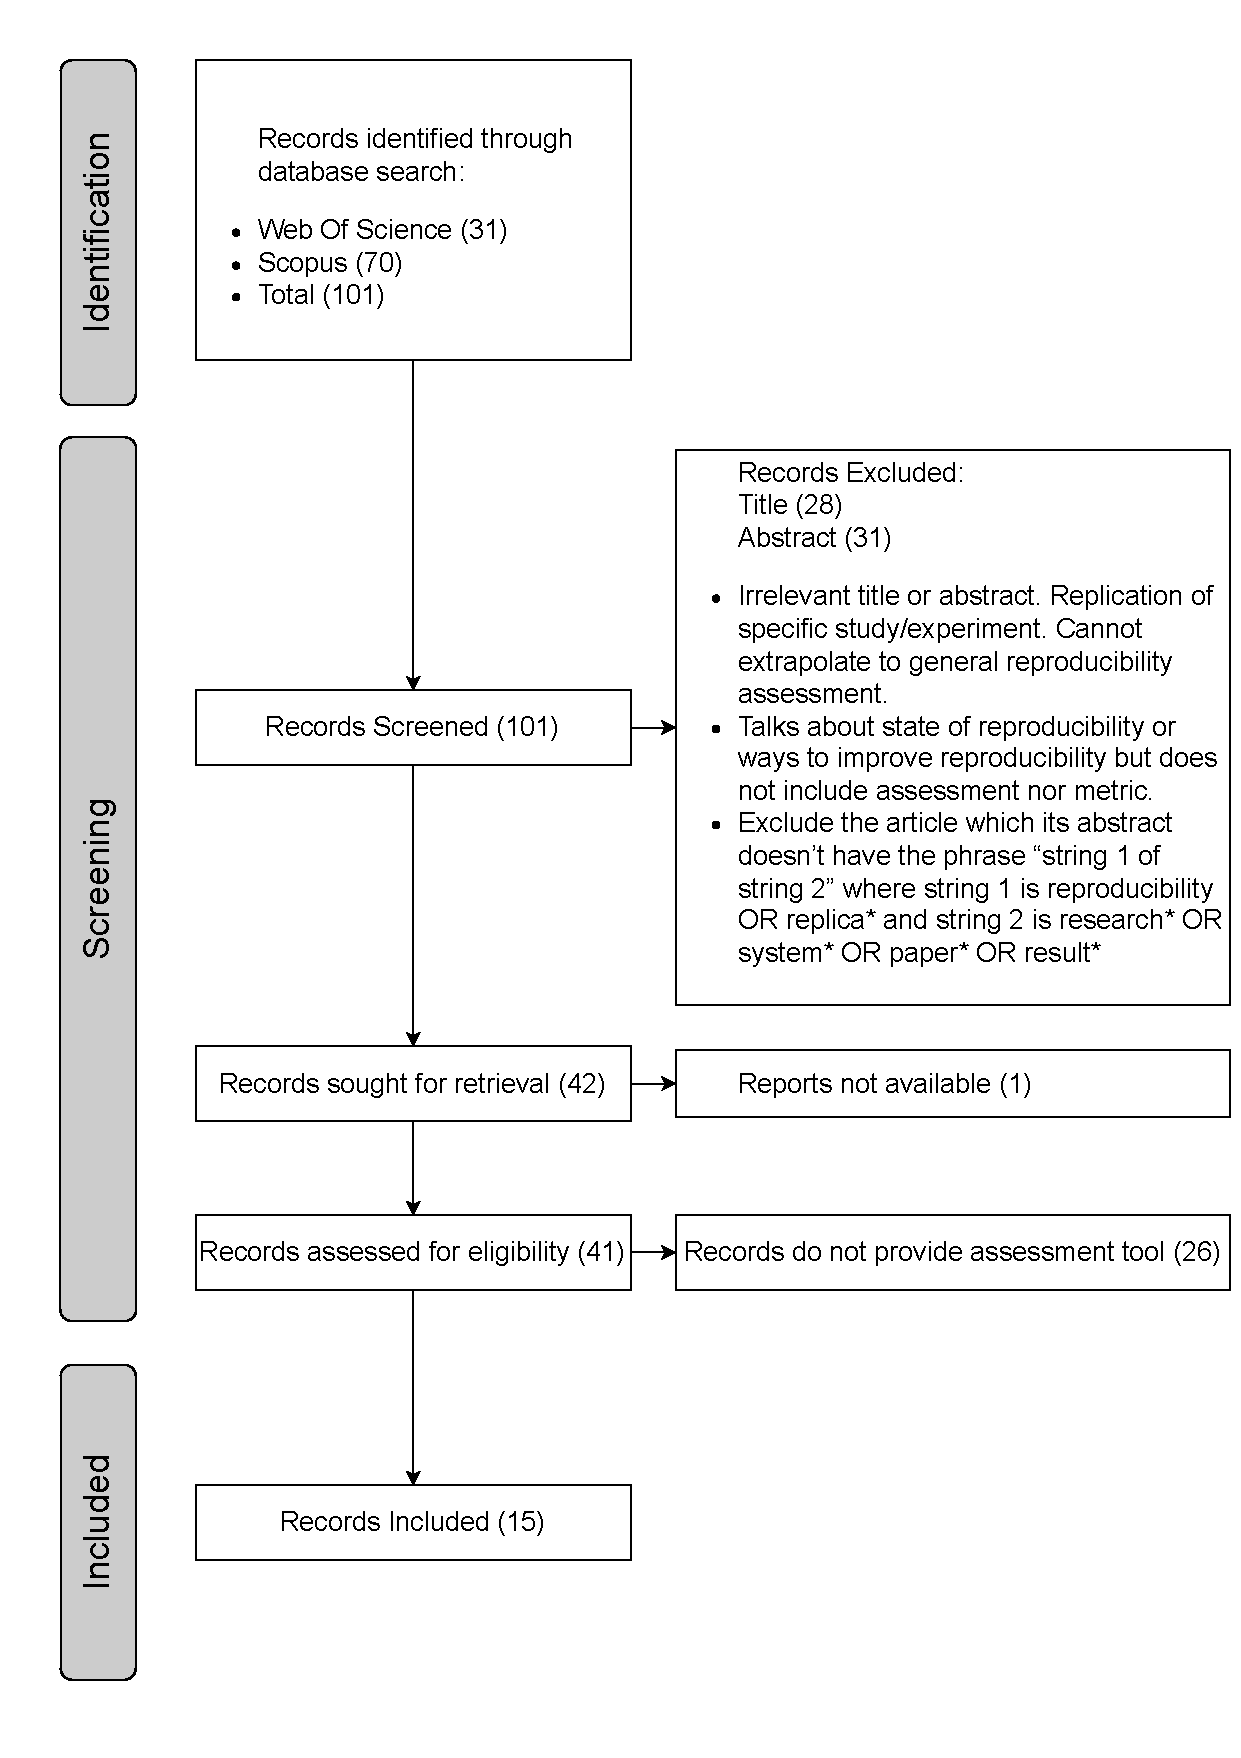
\includegraphics{prisma.pdf}}
				\caption[Prisma Flowchart]{Prisma Flowchart} 
				\label{fig:prisma}
			\end{figure*}



	The search criteria for the literature review were scientific papers or projects that assessed replicability using a model or algorithm that could be applied to scientific articles in general. The search was conducted across three databases: Web of Science, Scopus, and Engineering Village. The search strings shown in \tabref{tab:search_string_table} differ slightly because of the syntax of each database.

	\begin{table*}[htbp]
		\centering
		\caption[Search string for each database]{Search string for each database and number of hits retrieved (\#).}\label{tab:search_string_table}
		\small
			\begin{tabular}{llp{0.6\textwidth}}
			\hline
			Database & \# & Search string \\ \hline
			Web of Science & 31 & TI=((reproducibility OR replicability) AND ((scien* OR research OR result OR findings OR learning OR AI OR artificial intelligence) AND (predict OR estimate OR assess))) \\ 
			Scopus  & 70 & ( TITLE ( ( assess OR assessing OR evaluate OR evaluating OR predict OR predicting OR measure OR measuring OR quantify OR quantifying OR estimate OR estimating ) PRE/5 ( reproducibility OR replica* ) ) OR TITLE ( "Research replication prediction" ) OR TITLE ( ( reproducibility OR replica* ) W/3 ( "AI" OR "Artificial Intelligence" ) ) AND ABS ( ( reproducibility OR replica* PRE/2 "of" PRE/2 research* OR system* OR paper* OR result* ) OR ( "Research replication prediction" ) ) ) OR ( TITLE-ABS-KEY ( ( "Prediction market" ) )  AND  TITLE-ABS-KEY ( ( assess  OR  assessing  OR  evaluate  OR  evaluating  OR  predict  OR  predicting  OR  measure  OR  measuring  OR  quantify  OR  quantifying  OR  estimate  OR  estimating )  PRE/5  ( reproducibility  OR  replicability  OR  replication ) ) )  \\ \hline
			\end{tabular}
	\end{table*} 

		It must be noted that one of the search results, \citet{raghupathi2022Reproducibility}, adopts the method from \citet{gundersen2018state}. These are grouped together as one method under the section \ref{sec:num_methods}.  

	\section{Methods for reproducibility assessment}\label{sec:methods}
	The methods described in these papers can be classified into human-based methods (1), survey methods (2), machine learning methods (5), and other numerical methods (2).

		\subsection{Prediction market}
			\citet{Dreber2015using} used prediction markets to predict the outcome of 41 studies from the Reproducibility Project Psychology. The prediction market is a human-based method that simulates trading. Participants would have access to the original study as well as information about the setup of the person or team working on the replication. Each participant was given a \$100 to bet. The participants then traded contracts that would be worth \$1 if the replication was successful or nothing otherwise. A threshold of 0.5 was chosen for the final price. A price above the threshold indicated the paper was reproducible. \citet{Dreber2015using} prediction market correctly predicted 25 out of the 41 studies (61\%) from RPP.
				
			\citet{Gordon2021} analyzed data from two large-scale forecasting projects that involved a total of 78 research teams. They first surveyed each team about their research methods, data, and results, and then asked a separate group of participants to make predictions about the replicability of the research based on the survey responses. The authors found that the predictions made by the participants were generally accurate, with a correlation between predicted and actual replicability of 0.38. They also found that prediction markets - in which participants bet on the likelihood of research replicability - outperformed individual predictions, with a correlation of 0.51.

			\citet{Forsell2019} presents a method for predicting the replication outcomes of social and behavioral science experiments. The authors propose a statistical model that takes into account various features of the original study, such as sample size, effect size, and statistical power, as well as features of the replication study, such as sample size and effect size. The authors found that their model was able to predict the replication outcomes of the Many Labs 2 study with high accuracy. Specifically, the correlation between the predicted and actual outcomes was 0.77, indicating a strong positive relationship between the two. Moreover, the model was able to correctly predict the outcome of replication for 23 out of the 28 experiments, resulting in an overall accuracy of 0.82.

			\citet{Camerer2016evaluating} presents a method for evaluating the replicability of laboratory experiments in economics. The authors propose a framework that involves three steps: (1) conducting a meta-analysis of the original study, (2) replicating the original study with a larger sample size, and (3) comparing the results of the replication study with the meta-analytic effect size of the original study. The quantified output performance of the method is measured through the Replicability Index (RI), which is a statistical measure that indicates the degree to which a replication study confirms the findings of the original study. The RI ranges from 0 to 1, with higher values indicating greater replicability. The authors applied their method to a set of nine laboratory experiments in economics and found that the RI ranged from 0 to 0.83, with a median value of 0.30. This indicates that the replicability of the experiments varied widely, with some experiments showing strong replicability and others showing little to no replicability.

	\subsection{Surveys}
	Three studies,  \citet{stagge2019assessing},  \citet{mcintosh2017repeat} and \citet{QualityOutputChecklist} were found to utilize survey methods to assess reproducibility. \citet{stagge2019assessing} focused on reproducibility in hydrology and water resources, testing 360 publications from hydrology journals with a 15-question survey. The survey included questions designed to prevent participants from continuing if critical resources were missing. \citet{stagge2019assessing} manually replicated 20 publications containing data, code, and directions according to the survey, but only 4 were successful. The code repository can be accessed at \url{https://zenodo.org/record/2562268}.
	
	\citet{mcintosh2017repeat} conducted a literature review to identify 119 binary and nominal variables that must be included for research to be reproducible. These variables focus on transparency and availability and take the form of questions. While their article mainly analyzes the feature selection process, there is no implementation of these variables to assess or predict reproducibility. Both surveys include questions related to bibliographic information, data availability, and accessibility, and \tabref{tab:survey_table} provides an overview of the covered topics.
	
	\citet{QualityOutputChecklist} propose a checklist that includes five domains: design and analysis, data and materials, results, conclusions, and reporting. Each domain includes several items that researchers should address in their research outputs. The quantified output performance of the method is measured through the Quality Output Checklist and Content Assessment (QuOCCA) score, which ranges from 0 to 100, with higher scores indicating higher quality and reproducibility. The authors applied their method to a set of 26 research outputs in the field of cognitive neuroscience and found that the QuOCCA scores ranged from 39 to 92, with a median value of 68.

	\citet{Johnson2021Evaluating} identified a sample of 100 articles published in five high-impact emergency medicine journals between 2017 and 2018. They then assessed each article using a standardized reproducibility and transparency checklist that included 29 items related to research design, data analysis, and reporting. The authors found that the average score for the 29 items was only 14 out of 29, indicating that the majority of articles had significant limitations in terms of reproducibility and transparency. The most common issues were related to the lack of detail in reporting statistical analyses, inadequate reporting of inclusion and exclusion criteria, and insufficient detail in reporting the research question or hypothesis.

	\citet{Gordon2021} suggest that the experts' ratings provided useful information about the replicability of the psychological studies. For the correlation coefficient between the experts' ratings of the likelihood of replication success and the actual success rates of the replication attempts was 0.29. This indicates a moderate positive correlation between the two variables. For the prediction accuracy, the experts' ratings correctly predicted the replication success of 65 out of 100 studies, resulting in an overall prediction accuracy of 65%. This means that the experts were correct in their predictions for about two-thirds of the studies.
	
	We list questionare of three surveys in \tabref{tab:survey_table_2} and  \tabref{tab:survey_table_3}



	
	\begin{table*}[]
	\centering
	\caption[]{Questions introduced by \citet{stagge2019assessing}. }\label{tab:survey_table}
	\begin{tabular}{>{\raggedright\arraybackslash}p{0.25\textwidth} >{\raggedright\arraybackslash}p{0.25\textwidth} >{\raggedright\arraybackslash}p{0.25\textwidth} p{1.55cm}}  
	\hline
	Question                                                                                            & Answers leading to next question                                                                                           & Answers ending survey                                  \\ \hline
	1. Assessor's Name                                                                                   & -                                                                                                                                    & -                                                                                              \\
	2. Journal Name                                                                                     & -                                                                                                                                       & -                                                                                            \\
	3. Article DOI                                                                                      &  -                                                                                                                                       & -                                                                                              \\
	4. Full paper citation                                                                               & -                                                                                                                                      &  -                                                                                             \\
	5. How accessible to users?                                                                         & Some or all                                                                                                                            & Not specified where, not applicable.  \\
	6. Where available?                                                                                 & All online                                                                                                                             & Third party, author, in article.       \\
	7. What is present?                                                                                 & Required: input data, directions, code/software. Optional: license, metadata, identifiers, hardware/software requirements, file format. & -                                       \\
	8. Comments on availability                                                                         & \multicolumn{2}{l}{Open response}                                                                                                                                                                                                                \\
	9. Do you estimate you and your readers could generate the available artifacts to generate results? & Yes, not Sure, not familiar with resources.                                                                                             & No                                                                                             \\
	10. Continue to reproduce results?                                                                  & Yes                                                                                                                                    & No                                    \\
	11. Do the outputs verify the published results?                                                    & Yes                                                                                                                                    & No                                    \\
	12. If yes, explain what made the work reproducible and other comments                              &               -                                                                                                                         &   -                                    \\
	13. If no, why did the reproducing work fail?                                                     &       -                                                                                                                                 &     -                                 \\
	14. Other comments on why reproducing work failed?                                                  &     -                                                                                                                                   &        -                               \\ 
	15. How many minutes did it take the user to complete the survey                & Open Response                                          & -                                                                     \\ \hline
	\end{tabular}
	\end{table*}

	\begin{table*}[]
	\centering
	\caption[]{Questions introduced by \citet{stagge2019assessing} and  \citet{mcintosh2017repeat} and \citet{QualityOutputChecklist}, we only use abbreviated framework in \citet{mcintosh2017repeat}. }\label{tab:survey_table_2}
	\begin{tabular}{>{\raggedright\arraybackslash}p{0.1\textwidth}>{\raggedright\arraybackslash}p{0.3\textwidth} >{\raggedright\arraybackslash}p{0.3\textwidth}>{\raggedright\arraybackslash}p{0.3\textwidth}}  
	\hline
	&\citet{stagge2019assessing}         & \citet{mcintosh2017repeat}   &\citet{QualityOutputChecklist} \\                     
        \hline
	Basic question                &Q1. Assessor's Name             &                                                        &Q0. Assessor's Name                        \\
	&Q2. Journal Name                                                    & Q1. Journal Name                                &Q0. Journal Name                        \\
	&Q3. Article DOI                                                       &  Q2. Article DOI                                 &                     \\
	&Q4. Full paper citation                              &          & \\               
	&			&              & Q0. Date            	                     \\  
      \hline
	Accesible and available &Q5. How accessible to users?   &Q4. Publication state database(s) source(s) of data?       & Q2. Are the prmary data accessible to independent researchers on a public website?  \\
	 &Q9. Do you estimate you and your readers could generate the available artifacts to generate results?     &Q5. Publication states database(s) source(s) of data in the following location (Not Stated /Supplementary materials / Body of Text)          &Q3. Is code used for the study available on a public website to allow for reproduction or analysis of data?                                  \\
&Q8. Comments on availability  &Q16. Is the finalized dataset shared?   & \\
&Q6. Where available?&Q17. Where is the finalized dataset shared?      & \\
&& Q18. Is there a clear process for requesting the data?  & \\
	\hline
What is present &Q7. What is present?          &Q6. Query methodology (Manual extraction/Digital extraction through query interface / Digital extraction through honest broker / Not Applicable / Not Stated)  &\\
&&Q7. Does the shared query script for database contain comments and/or notations for ease of reproducibility?&\\
&& Q13. Does the author state analysis methodology and process?                                 & \\
&& Q14. Does the author indicate the software used to develop the analysis code? & \\
&& Q15. Is the analysis software proprietary or open? & \\ 

\hline

	\end{tabular}
	\end{table*}


	\begin{table*}[]
	\centering
	\caption[]{\textbf Questions introduced by \citet{stagge2019assessing} and  \citet{mcintosh2017repeat} and \citet{QualityOutputChecklist}, we only use abbreviated framework in \citet{mcintosh2017repeat}. }\label{tab:survey_table_3}{\textbf{Table 4 Continued:}}
	\begin{tabular}{>{\raggedright\arraybackslash}p{0.12\textwidth}>{\raggedright\arraybackslash}p{0.3\textwidth} >{\raggedright\arraybackslash}p{0.3\textwidth}>{\raggedright\arraybackslash}p{0.28\textwidth}}  
	\hline
&	\citet{stagge2019assessing}                                                                           & \citet{mcintosh2017repeat}        					 &\citet{QualityOutputChecklist}                   \\ 
\hline
Data Processing / Analysis
&&Q8. Does the research involve natural language processing or text mining?   &Q9a. Were any data excluded? 		\\
&&Q9. Please list all software applications used for text mining  &Q9b. If so, was a criterion given? \\
&&Q10. Please enter all that apply separated by a semicolon&Q6. Was data analysis blinded?\\
&&Q11. Does the publication clearly state process(es) for validating data minded via nlp and/or queried from a database?      &Q8a. Are all measures of variability defined in figures, tables and text?		 \\
&&Q3. Is the research hypothesis-driven or hypothesis-generating?           &Q8b. Are any data summarised using standard error of the mean (SEM)? 		\\
&&&Q8c. If the SEM is used, are sample sizes specified for all reported SEM?            \\
&&&Q1a. Were the study's hypotheses and analyses plans registered prior to the conduct of the study (i.e. pre-registered)?   \\
&&&Q1b. If so. was the main conclusion reported in the abstract (or summary) based on the primary hypothesis/outcome?     \\
&&&Q10a. If null-hypothesis testing of significance was used, is a probability threshold specified for all statistical tests?	\\
&&&Q10b. If used, are exact probability values used throughout the report, excluding figure legends ? \\
&&&Q5a. Was the sample size based on a formal sample size calculation done prior to starting the study? 	                      \\
&&&Q5b. If so, was the planned sample size adhered to?    \\	 
\hline
	\end{tabular}
	\end{table*}

	\begin{table*}[]
	\centering
	\caption[]{\textbf Questions introduced by \citet{stagge2019assessing} and  \citet{mcintosh2017repeat} and \citet{QualityOutputChecklist}, we only use abbreviated framework in \citet{mcintosh2017repeat}. }\label{tab:survey_table_3}{\textbf{Table 4 Continued:}}
	\begin{tabular}{>{\raggedright\arraybackslash}p{0.1\textwidth}>{\raggedright\arraybackslash}p{0.3\textwidth} >{\raggedright\arraybackslash}p{0.3\textwidth}>{\raggedright\arraybackslash}p{0.3\textwidth}}  
	\hline
&	\citet{stagge2019assessing}                                                                           & \citet{mcintosh2017repeat}        					 &\citet{QualityOutputChecklist}                   \\ 
\hline
Result 
&Q10. Continue to reproduce results?& &Q11. Are claims made for the importance or significance of results associated with a revalue greater than or equal to 0.05(or other threshold) i.e. misleading spin of reported results ? \\
&Q11. Do the outputs verify the published results? 		&&\\
&Q12. If yes, explain what made the work reproducible and other comments. 	&&\\
&Q13. If no, why did the reproducing work fail?&&\\
\hline
Other &Q14. Other comments on why reproducing work failed?         &Q11. Is the text mining software application proprietary or open?&Q4. Was ethics approval obtained?              \\     
&Q15. How many minutes did it take the user to complete the survey  &Q12. If multiple applications were used, please select all options that apply.    &Q7. Are any reporting guidelines specified (such as those found at www.equator-network.org)?     \\                  
\hline

	\end{tabular}
	\end{table*}


		\subsection{Machine learning methods}\label{sec:ML_methods}

			\subsubsection{NLP methods}\label{sec:NLP_methods}
			
			 \citet{Yang2020estimating} and \citet{luo2020research} developed machine learning models that use features derived from text to evaluate the reproducibility of scientific papers. \citet{Yang2020estimating} presented three models: a text-only model, a metric-based model, and a text and metric model. The text-only model uses paper-level vector representations fed to an ensemble of random forests with bagging and logistic regression. The papers are stripped of non-textual content such as authors, citations, figures, and graphs. Then, a Word2Vec neural network transforms words into vectors that retain semantic information. Yang trained Word2vec on the Microsoft Academic Graph papers as a corpus to produce 200-dimensional vectors.
			
			Then the term frequency (TF) and inverse document frequency (IDF) are calculated. The TF is defined as the number of times a term ($W_{i}$) appears in a paper divided by the total number of terms in the paper ($W_{T}$).

			\begin{equation}  
				TF = W_{i}/W_{T}              
			\end{equation}			

			\noindent The IDF is defined as the logarithm of the total number of documents in a collection ($D_{T}$) divided by the number of documents that contain the term in question ($D_{i}$).  

			\begin{equation}
				IDF = log(D_{T}/D_{i})
			\end{equation}
			
			\noindent To generate a metric for assessing the reproducibility of scientific papers, \citet{Yang2020estimating} utilized term frequency-inverse document frequency (TF-IDF). First, they calculated the term frequency (TF), which is the number of times a term ($W_{i}$) appears in a paper divided by the total number of terms in the paper ($W_{T}$). Then, they calculated the inverse document frequency (IDF), which is the logarithm of the total number of documents in a collection ($D_{T}$) divided by the number of documents that contain the term in question ($D_{i}$). The IDF helps identify how unique a term is to a document in the context of a collection of documents. Terms that appear in only a small number of documents receive a high IDF, while terms that appear in many documents receive a low IDF value. To generate a combined metric, TF is multiplied by IDF, yielding the metric TF-IDF.

			\begin{equation}
				\textit{TF-IDF} = TF * IDF
			\end{equation}

			In the TF-IDF method, the term frequency and inverse document frequency are multiplied by the corresponding word vectors from Word2vec to generate two features: a TF vector and a TF-IDF vector. These features represent the paper and are fed to an ensemble of random forests with bagging and bagging with logistic regression. The model outputs a prediction of either 0 for failed or 1 for passed. The model was trained on the 96 papers from the Reproducibility Project Psychology and achieved an average accuracy of 0.68 and top k precision of 0.75 after 100 rounds of three-fold cross-validation.

			\citet{luo2020research} proposed a weakly supervised learning model to predict the reproducibility of scientific articles. The process starts with extracting text from PDFs, followed by converting the text to features using either TF-IDF for bag-of-word models or word embeddings using Bidirectional Encoder Representations from Transformers (BERT) for sequential models. Weakly supervised learning is used due to the lack of labeled data (studies with manually replicated reproducibility outcomes). First, a model is trained with labeled data, and then unlabeled data is fed to generate "noisy labels" for the unlabeled data. The authors propose two approaches to deal with the noisy labels: Variational Inference aided Weakly Supervised Learning and Peer Loss aided Weakly Supervised Learning. These methods differ in the way noisy labels are aggregated and the loss function used for the LSTM network, but follow a similar workflow otherwise. First, five classifiers (logistic regression, random forests, support vector machines, multilayer perceptron, and long short-term memory) are trained on labeled data. Then the trained classifiers are fed all of the training data (labeled and unlabeled) to produce noisy labels. This is where the approaches diverge.
			
			Variational inference aided weakly supervised learning adopts a method proposed by \citet{Liu2012VariationalIF} to estimate error rates of the noisy labels. This model correctly predicted 66 out of 99 papers (67\%). The peer loss-aided weakly supervised learning method uses a majority voting rule for the noisy labels. Two other random samples (peers) are randomly drawn and used as input for the peer loss function. The LSTM network is trained using a peer loss function from \citet{liu2020peer}. This method predicted 71 papers out of 99 (71\%).

%			\begin{figure*}[t]
%				\centering
%				\includegraphics[width=\columnwidth]{Luo2020_var_inference.png}
%				\caption[Variational Inference Flowchart]{Variational Inference Flowchart} 
%				\label{fig:var_inference}
%			\end{figure*}

%			\begin{figure*}[t]
%				\centering
%				\includegraphics[width=\columnwidth]{Luo2020_peer_loss.png}
%				\caption[Peer Loss Flowchart]{Peer Loss Flowchart} 
%				\label{fig:peer_loss}
%			\end{figure*}

			Two machine learning methods for predicting the reproducibility of scientific articles are described in this section. Variational inference aided weakly supervised learning is a method proposed by \citet{Luo2022sentence} that estimates error rates of noisy labels to successfully predict 66 out of 99 papers (66\%). The peer loss-aided weakly supervised learning method uses a majority voting rule for the noisy labels and predicted 71 out of 99 papers (71\%). \citet{Luo2022sentence} developed an explainable machine learning model called "Variational Contextual Consistency Sentence Masking (VCCSM)" to predict reproducibility. The model identifies important sentences in predicting reproducibility by feeding the text from a paper to an LSTM model, which omits some sentences at random. During training, the model learns to produce masks that minimize noise and maximize information for prediction. VCCSM is a semi-supervised learning method that uses the same dataset as \citet{Luo2022sentence} but relies only on the LSTM model. The authors tried two embeddings, Google pre-trained embeddings and BERT pre-trained embeddings, and found that the BERT version achieved better performance.
			

			\subsubsection{Methods using directly derived statistics as features}
			\citet{Altmejd2019predicting} utilized machine learning methods to predict replicability based on 68 features such as p-values, number of citations, effect size, and authors. They employed two techniques: a random forest and regression. The regression model aimed to predict the "relative effect size estimate," defined as the replication effect size divided by the original effect size, where the effect size appears in the dependent variable but is also used as an independent variable. The regression model had a root mean squared error of 0.51, while the random forest model achieved an accuracy of 0.69. Tables containing all variables and their descriptions are available in their supplementary materials.
			
			\citet{wu2021predicting}, which describes a framework called FEXRep for extracting features to assess the reproducibility of scientific papers. FEXRep uses machine learning tools and bibliographic APIs to extract 41 features that can be classified as bibliometric, venue-related, author-related, statistical, and semantic. To extract features such as authors and digital object identifier (DOI), FEXRep takes documents in PDF format as input, and uses GROBID, a machine learning library that extracts bibliographic information from scientific articles. To find p-values, the PDFs are first converted into text using PDFTOTEXT, and then regular expressions are used.
			

			The paper describes a literature review of methods to assess reproducibility in scientific research. Reproducibility is defined as obtaining consistent computational results using the same input data, computational steps, methods, code, and conditions of analysis. The authors used the PRISMA 2020 standard to conduct their literature review and found ten relevant articles that describe methods to assess reproducibility. The methods are classified into human-based, survey-based, machine learning-based, and numerical categories. While the machine learning methods are promising, none of the reviewed models achieved an accuracy above 75\%. The authors suggest that transformer models, a state-of-the-art architecture used in natural language processing, could be effective in predicting reproducibility. The paper also provides an overview of the most important features identified by \citet{wu2021predicting} for assessing reproducibility, including self-citations, author count, influential references count, reference result, number of hypotheses tested, upstream influential methodology count, influential citation count, average author citations, and citation methodology. The support vector machine algorithm had the best-reported performance with an F1 score of 0.68 and recall of 0.99, while the quadratic discriminant analysis had the best precision (0.69).

		\subsection{Other numerical methods} \label{sec:num_methods}

			 The numerical methods mentioned in this section are different from the machine learning methods because these don’t use data nor perform any type of training or fitting. The two methods in this section are Quantified reproducibility assessment of NLP results by \citet{belz2022quantified} and Reproducibility of experiments, data, and methods by \citet{gundersen2018state}. 

			\citet{belz2022quantified} propose a reproducibility assessment method inspired in metrology which consists of taking the same measurement several times and then calculating the precision (how close or far are the measurements from one another) of the set of measurements. In the paper, the method is adapted specifically for natural language processing tasks.

			To summarize, precision can be calculated using metrics such as the mean value or 95\% confidence interval, and this metric is taken as the reproducibility score. For reproducibility assessment, a model (code) to test and an evaluation method (e.g., BLEU for NLP tasks) are needed. In this case, the authors used a coefficient of variation (CV) as the precision metric.
			\begin{equation}\label{cv}
				CV = \frac{1}{m} \frac{\sqrt[]{\frac{S}{DoF}}}{\sqrt[]{\frac{2}{DoF}} \Gamma(\frac{s}{2})  \Gamma(\frac{DoF}{2}) }
			\end{equation}


			\noindent The numerator is defined as the square root of the sum of squared differences (S) divided by the degrees of freedom (DoF). Additionally, in the denominator, the mean (m), sample size (s), and the gamma distribution ($\Gamma$) are used.


			\citet{gundersen2018state} use a numerical method to calculate the reproducibility of experiments, methods, and data depending on the results of their survey. The variables are a set of survey items that take a value of 0 or 1 if they are explicitly mentioned in the paper or not. The items belong to one of the three categories: experiments, methods, and data. For example, the data-related items chosen by \citet{gundersen2018state} are training data,  validation data, test data, and results. If a paper provides training data, then this variable will have a value of 1. These variables were manually extracted by reading the papers to be assessed. The idea is to assess different levels of reproducibility. The reproducibility of methods depends only on the variables pertaining to the methods, so it is the most general level. The reproducibility of the data depends on the variables from the methods and the data. Finally, the reproducibility of the experiment depends on the variables from all three areas. After the binary values are obtained, the reproducibility scores for experiments ($R_{E}$), data ($R_{D}$), and methods ($R_{M}$) are defined in terms of the variables for the methods (M), data (D), and experiments (E) according to the following equations:

			\begin{equation}
				R_{E} = \frac{\delta_1*M + \delta_2*D + \delta_3*E}{\delta_1 + \delta_2 + \delta_3}
			\end{equation}

			\begin{equation}\label{data_eq}
				R_{D} = \frac{\delta_1*M + \delta_2*D }{\delta_1 + \delta_2}
			\end{equation}

			\begin{equation}
				R_{M} = M 
			\end{equation}

			\textit{E}, \textit{D}, and \textit{M} are calculated in terms of the percentage of variables present. For example, if two out of the four items for data are present, then the term $D$ in \eqref{data_eq} takes a value of 0.5. \citet{gundersen2018state} uses all $\delta = 1$. Each paper has three reproducibility scores: experiment reproducibility, method reproducibility, and data reproducibility. 

			\citet{Breuer2020} suggest that the proposed method can be used to quantitatively measure the reproducibility of system-oriented IR experiments and identify factors that affect reproducibility. The authors calculated the Repeatability Score (RS) and Reproducibility Score (RP) for three different metrics: Mean Average Precision (MAP), Precision at 10 (P@10), and Recall. The RS for MAP was 0.91, indicating high repeatability, while the RP was 0.59, indicating moderate reproducibility. For P@10, the RS was 0.79, indicating moderate repeatability, and the RP was 0.46, indicating low reproducibility. Finally, for Recall, the RS was 0.71, indicating moderate repeatability, and the RP was 0.53, indicating low reproducibility.

			The methodology of \citet{Ang1998} involves splitting the data into multiple random samples and using one sample to build a regression model while the others are used to validate the model. This process is repeated multiple times, and the results are averaged to obtain a more robust estimate of the model's performance. The bootstrap method is used to generate confidence intervals around the estimated performance metric. The authors applied this methodology to a dataset of 61 variables predicting a target variable of interest. They compared the results of their methodology to those obtained from a traditional split-sample approach. They found that the double cross-validation and bootstrap method resulted in more stable and reliable estimates of the model's performance. The quantified output performance reported in the article includes the mean and standard deviation of the estimated performance metric (R-squared) across the multiple iterations of the methodology, as well as the 95% confidence intervals generated by the bootstrap method. The authors also reported the percentage of times each variable was selected as significant in the regression model across the multiple iterations.

			\citet{Ang1998Evaluate}proposes a method for assessing the replicability of results by using the jackknife statistic. The jackknife is a resampling method that involves systematically leaving out one or more observations from a dataset and refitting the model. This process is repeated for each observation in the dataset, resulting in a set of estimates of the model's parameters. The authors applied the jackknife method to a dataset of 54 variables predicting a target variable of interest. They used the jackknife to estimate the model's parameters and compared the results to those obtained from a traditional split-sample approach. They found that the jackknife method resulted in more stable and reliable estimates of the model's parameters and better replicability of the results.

			\citet{Thompson2006} used a qualitative approach to evaluate the replication of each study by comparing the results of the replication study to the original study's results. They used a statistical significance criterion of p < 0.05 to determine whether the replication study produced a statistically significant result in the same direction as the original study. The quantified output performance reported in the article includes the percentage of studies that replicated the original results and the effect size of the replication. The authors found that only 36% of the studies were successfully replicated, indicating a significant replication crisis in psychology. They also found that the effect size of the replications was on average about half the size of the original studies, suggesting that the original studies may have overestimated the true effect size.

			\citet{Estimatingthereplicability} used a systematic review method to assess the replicability of research in technology education. The authors identified 225 articles published between 2010 and 2018 in three major technology education journals, and rated each article on 13 criteria related to research design, analysis, and reporting. The authors found that the average score for the 13 criteria was 7.1 out of 13, indicating that the majority of articles had significant limitations in terms of their replicability. The most common issues were related to the lack of detail in the reporting of methods and results, the lack of clarity in the research questions and hypotheses, and the inadequate reporting of statistical analyses. The authors concluded that the replicability of technology education research is low and that there is a need for greater attention to be paid to research design, analysis, and reporting in this area.

	\section{Results and Discussion} \label{sec:Results}
		One of the main challenges in assessing reproducibility in science is the lack of a clear and widely accepted definition and metric for determining the reproducibility of an article. This can be problematic for supervised machine learning algorithms, which rely on labeled data for training. Our literature review found that the most common criterion for reproducibility is based on the replication's p-value and effect size. If the replication results yield a p-value less than 0.05 and the effect size is in the same direction as the original study, then the study is considered reproducible. If the replication results fail to meet these two conditions, then the study is considered irreproducible. This criterion is adopted by two projects and four of the methods reviewed in this literature review.

While survey methods are the simplest to use, they still require individuals to read through the documents and identify survey items. \citet{stagge2019assessing} was only able to reproduce 4 out of 20 papers that met all the criteria in their survey. \citet{gundersen2018state} starts as a survey and then takes steps to numerically quantify the reproducibility of a paper's experiments, data, and methods, but does not propose a threshold for reproducibility and does not utilize any of the reproducibility datasets in \tabref{tab:datasets_table}. \citet{belz2022quantified} method only applies to articles with available data, code, and well-defined evaluation metrics.

Machine learning methods suffer from a lack of large enough datasets. The methods in \ref{sec:NLP_methods} use data from reproducibility projects which are expensive, time-consuming and uncommon. \citeyear{Yang2020estimating} gathered the most samples (n=413).  \tabref{tab:performance_table} shows the performance of these methods. \citet{Luo2022sentence} achieved the highest accuracy (0.75). These are the only two methods that use a natural language processing (NLP) approach to extract features from text. \citeyear{Yang2020estimating} generated features by multiplying Word2Vec word vectors with term frequency-inverse document frequency (TF-IDF) values, while \citet{Luo2022sentence} used BERT's pre-trained embeddings as features.  \citeyear{Altmejd2019predicting} and  \citeyear{wu2021predicting} used hand-picked statistics as features.

	 

		\begin{table*}[ht]
		\centering
		\caption[Datasets]{Datasets used by ML methods}\label{tab:datasets_table}
		\begin{tabular}{p{0.41\linewidth} p{0.08\linewidth} p{0.08\linewidth} p{0.08\linewidth}  p{0.08\linewidth} p{0.08\linewidth}} 
		\hline
		\centering\arraybackslash{Dataset name}                                                          & \citet{Yang2020estimating} & \citet{Altmejd2019predicting} & \citet{wu2021predicting} & \citet{luo2020research} & \citet{Luo2022sentence} \\ \hline
		\citet{Klein2014data}                                                                                            & yes                        & yes                           & yes                                                 & yes                               & yes                    \\ 
		\citet{Open2015estimating}                                                   & yes                        & yes                           & yes                                                                                 & yes                               & yes                    \\
		\citet{Ebersole2016many}                                                                                           & yes                        & yes                           & no                                             & yes                               & yes      \\
		\citet{Camerer2016evaluating}                                     & yes                        & yes                           & no                                                                                            & yes               & yes      \\ 
		\citet{Klein2018many}                                                                                           & yes                        & no                            & yes                                                 & yes            & yes         \\ 
		\citet{Camerer2018evaluating}                                                  & yes                        & no                            & no                                                                               & yes              & yes       \\ 
		Registered Replication Report$^{1}$                                                         & yes                        & no                            & no                                                               & yes              & yes       \\
		Curate Science$^{2}$                                                                                       & yes                        & no                            & no                                                      & no              & no         \\
		PsychFileDrawer$^{3}$                                                                                   & yes                        & no                            & no                                                        & yes               & yes      \\
		Economics Replication Wiki$^{4}$                                                          & yes                        & no                            & no                                                                  & no                & no       \\ \hline
		\end{tabular}
		    \begin{tablenotes}
		      \small
		      \item \raggedright\arraybackslash\tiny Links: $^{1}$\url{https://www.psychologicalscience.org/publications/replication}, $^{2}$\url{https://curatescience.org/app/home/}, $^{3}$Not accessible, $^{4}$\url{https://replication.uni-goettingen.de/wiki/index.php/Main_Page} (last accessed 2022-11-04).
		    \end{tablenotes}
		
		\end{table*}


	\begin{table*}[ht]
		\centering
		\caption[Performance Table]{The best model for each ML method. The inputs are text or statistics (stats). The metrics used are accuracy (Acc), F1 score, recall (Re), area under the perturbation curve (AUPC), and post-hoc accuracy (Post Acc). The total number of studies used for training (\#T), number of studies for validation (\#V), number of folds in cross-validation$^{f}$, and number of unlabeled studies$^{u}$ in semi-supervised learning is shown in the last two columns.}\label{tab:performance_table}
		\begin{tabular}{>{\raggedright\arraybackslash}p{0.19\linewidth} >{\raggedright\arraybackslash}p{0.15\linewidth} >{\raggedright\arraybackslash}p{0.19\linewidth} >{\raggedright\arraybackslash}p{0.17\linewidth}  c c}  
		\hline
		ML method                     & Input               & Best model                             & Performance                                           &  \#T  & \#V       \\ \hline

		\citet{Yang2020estimating}    				& Text and stats 	& Random forest and logistics regression & Acc 0.71                    & 96 (3$^{f}$)   & 317 \\ 
		\citet{Altmejd2019predicting} 		& Stats          	& Random forest                          & Acc 0.71                                            & 131 (5$^{f}$)     &    \\ 
		\citet{wu2021predicting}     			& Stats          	& SVM                                    & F1 0.68, Re 0.99                                & 139 (5$^{f}$)   &  \\ 
		\citet{luo2020research}       				& Text and stats 	& Peer loss model                        & Acc 0.75                                       & 300+2170$^{u}$	& 99   \\ 
		\citet{Luo2022sentence}     				& Text		& VCCSM                                       & Acc 0.68, AUPC 0.24, Post Acc 0.65 & 300+2170$^{u}$	& 99\\ \hline                                      
		\end{tabular}				
	\end{table*}


%	\section{Results}
%	We previously tried to replicate\citet{Yang2020estimating} text-only model, but due to a lack of accessibility to all the articles used for training, no available code, as well as some doubts about the implementation details of their model, we have been unsuccessful in our endeavor.
% 
%The training set consists of  96 papers from RPP. Less than half of these publications have open access. We searched through the entire list of publications, and when they were unavailable, we requested access from the author. Including the authors that responded and shared their publications, we only managed to gather 48 articles. There was no information or benchmarks on their word2vec model which made it impossible to compare it to a word2vec model trained on another corpus. We were unclear about some of the details in the implementation of their model. There is no mention of the source code in the main publication or the appendix. We contacted the authors but did not receive their data or source code.


	\section{Conclusion} \label{sec:conclusion}
The review concludes that more research and development is needed to improve the state of reproducibility in science. The literature review examined ten methods for assessing reproducibility, with varying degrees of complexity and rigor. Machine learning methods were found to be the most promising option, due to the inherent need for testing and validation in the field. The NLP methods discussed all used some way of representing text as vectors, but then used either a machine learning algorithm or an LSTM neural network for prediction. No article in the literature was found to use a transformer model for prediction, most likely due to the scarcity of labeled reproduced articles. However, the authors propose that transformer models, which are state-of-the-art in NLP and to a lesser extent in computer vision, would be effective for predicting reproducibility. The attention mechanism used in transformer models excels at learning relationships between elements within a set and can calculate attention for all elements in a single operation, unlike older architectures such as recurrent neural networks where elements are processed sequentially.


	\section{Acknowledgments}
	We express our gratitude towards the Ministry of Science and Technology in Taiwan for their financial support under grants MOST 110-2222-E-006-010 and 111-2221-E-006-186. We would also like to acknowledge the valuable input received from various individuals, Akram Ashyani, Jose Ramon Chang, Ray Chen, Esteban Roman Catafau, Rain Wu, Gavin Vivaldy, Jacob Chen, Ric Tu, Yu-Shan Lin, Austin Su, Benson Feng, Hen-Sue Kung, Jagmohan Meher, Alvin Anderson, Vu Cong Thanh, Nguyen Ba Tho, Tran Quang Huy, Jiří Filip, Omar Hernandez, Alan Tsai, Ai-Yung Chen, Howard Liu, Samuel Chen, and OpenAI.

	\section{Declarations}
	The authors declare no conflict of interest exists.

	\clearpage

	\section{References} \label{sec:references}
		%% Select the correct font size to fit within page limit
		%\normalsize
		%\small
		\footnotesize
		%\scriptsize
		%\tiny
	\bibliography{../LibraryAllReferences} %Can be placed anywhere within section 3 
	%\clearpage

	
	\onecolumn	
	\section{Appendix}\label{sec:Appendix}
	
	All the relevant articles are listed in Table \ref{tab:allarticles}.


	
	\begin{table*}[h!]
	%\centering
	\caption[]{All the article we found. \label{tab:allarticles}}
	\begin{tabular}{>{\raggedright\arraybackslash}p{0.15\textwidth}>{\raggedright\arraybackslash}p{0.75\linewidth}}  
	\hline
	Citation                     & Title           \\ \hline
	\citet{Dreber2015using}  &Using prediction markets to estimate the reproducibility of scientific research \\
%	\\
	\citet{stagge2019assessing}  &Assessing data availability and research reproducibility in hydrology and water resources \\
%	\\
	\citet{mcintosh2017repeat}  &Repeat: a framework to assess empirical reproducibility in biomedical research \\
%	\\
	\citet{Yang2020estimating}  &Estimating the deep replicability of scientific findings using human and artificial intelligence \\
%	\\
	\citet{luo2020research}  &Research replication prediction using weakly supervised learning. \\
%	\\
	\citet{Luo2022sentence}  &Interpretable Research Replication Prediction via Variational Contextual Consistency Sentence Masking \\
%	\\
	\citet{Altmejd2019predicting}  &Predicting the replicability of social science lab experiments \\
%	\\
	\citet{wu2021predicting}  &Predicting the Reproducibility of Social and Behavioral Science Papers Using Supervised Learning Models \\
%	\\
	\citet{belz2022quantified}  &Quantified Reproducibility Assessment of NLP Results \\
%	\\
	\citet{Gordon2021}   &Predicting replicability-Analysis of survey and prediction market data from large-scale forecasting projects \\
%	\\
	\citet{Breuer2020}  &How to Measure the Reproducibility of System-oriented IR Experiments \\
%	\\
	\citet{NIMS2017750}  &Assessing reproducibility in faunal analysis using blind tests: A case study from northwestern North America \\
%	\\
	\citet{Forsell2019}  &Predicting replication outcomes in the Many Labs 2 study  \\
%	\\
	\citet{gundersen2018state}  &State of the Art: Reproducibility in Artificial Intelligence \\
%	\\
	\citet{Johnson2021Evaluating}  &Evaluating Reproducibility and Transparency in Emergency Medicine Publications \\
%	\\ 
	\hline

	\end{tabular}
	\end{table*}


	

	
\end{document}      % End of the document
 